%!TEX root = ../these.tex

\subsection*{%
Решение задач большой размерности
}
\label{sec:pcgtsp.ufa}

Предлагаемый алгоритм существенно увеличивает размеры
экземпляров задач PCGTSP,
для которых может быть получено точное решение с
$\approx 30$
\cite{bi:RoMa}
до 50--60,
а в некоторых случаях до
$\approx 150$
(в зависимости от вложенности контуров).
Вместе с тем,
задачи большой размерности
(сотни и тысячи контуров)
все еще остаются недоступными для точного
решения
(за разумное время),
однако для них легко находятся
практически приемлемые решения.

Примеры таких маршрутов приведены на
рис.~\ref{fig:pcgtsp.ufa}.
Раскройные планы предоставлены
М.А.~Верхотуровым,
численные данные приведены
в~табл.~\ref{tab:pcgtsp.ufa}.

\begin{figure}
  \centering
  \subfloat[$m=424$ контура; $n=2062$ узла]{
    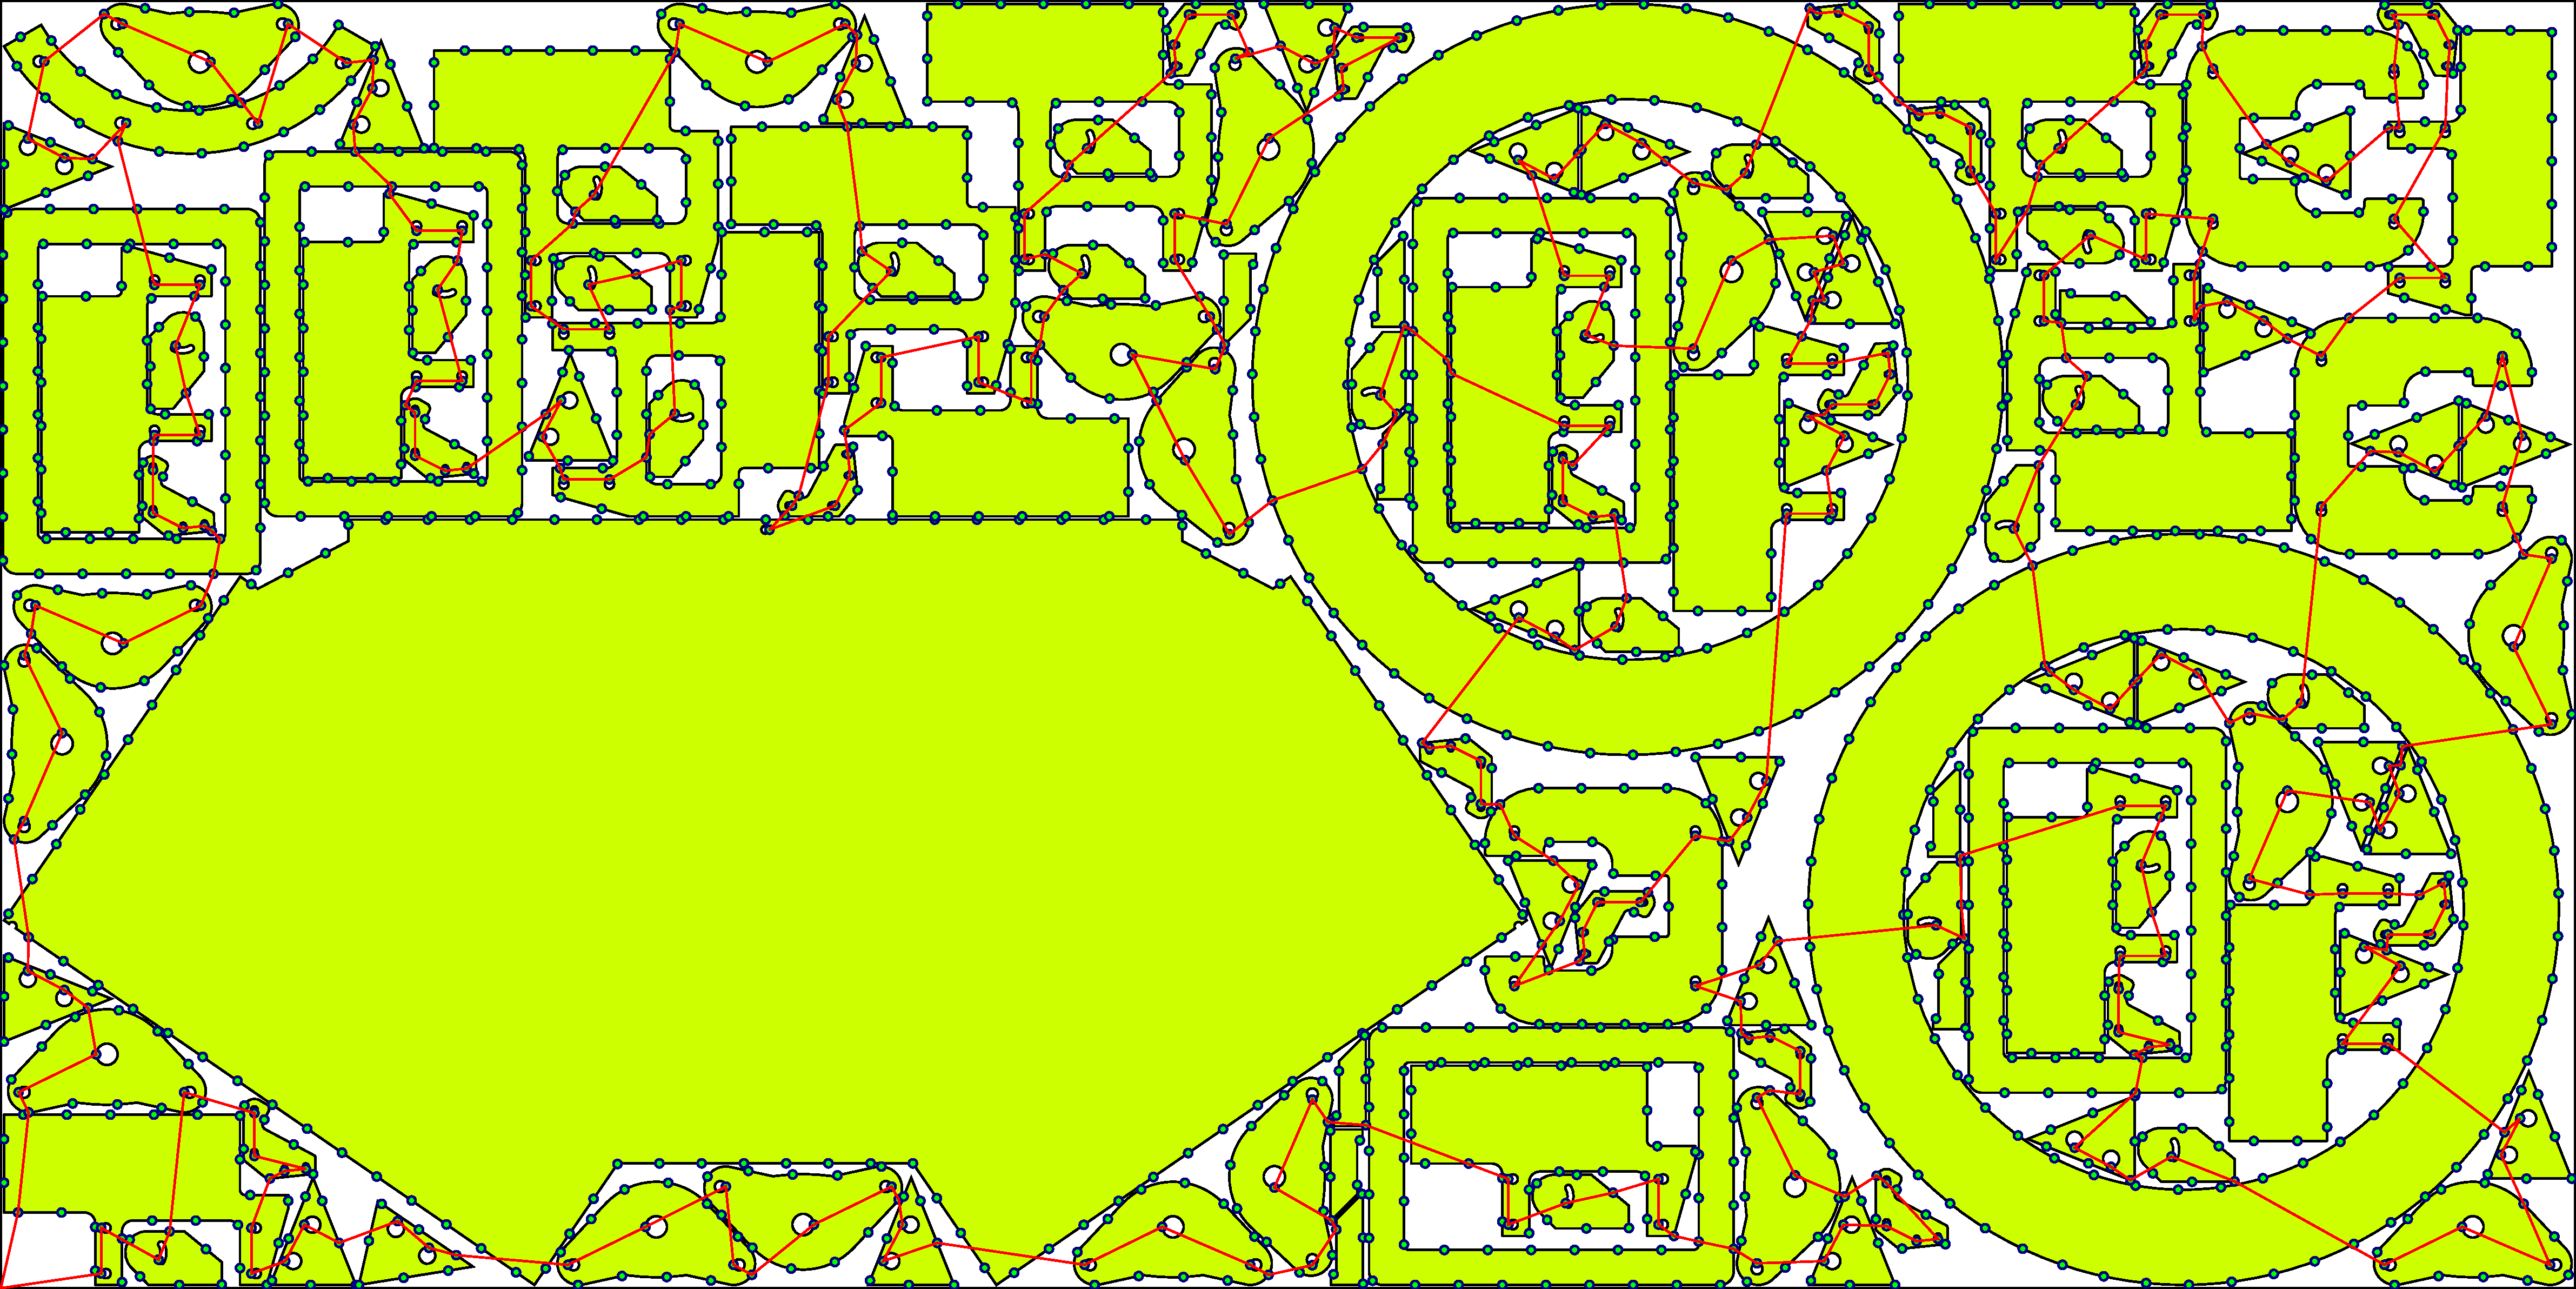
\includegraphics[width=0.95\textwidth]{ufa/a.pcglns.pdf}
  }
  \\
  \subfloat[$m=621$ контур; $n=2253$ узла]{
    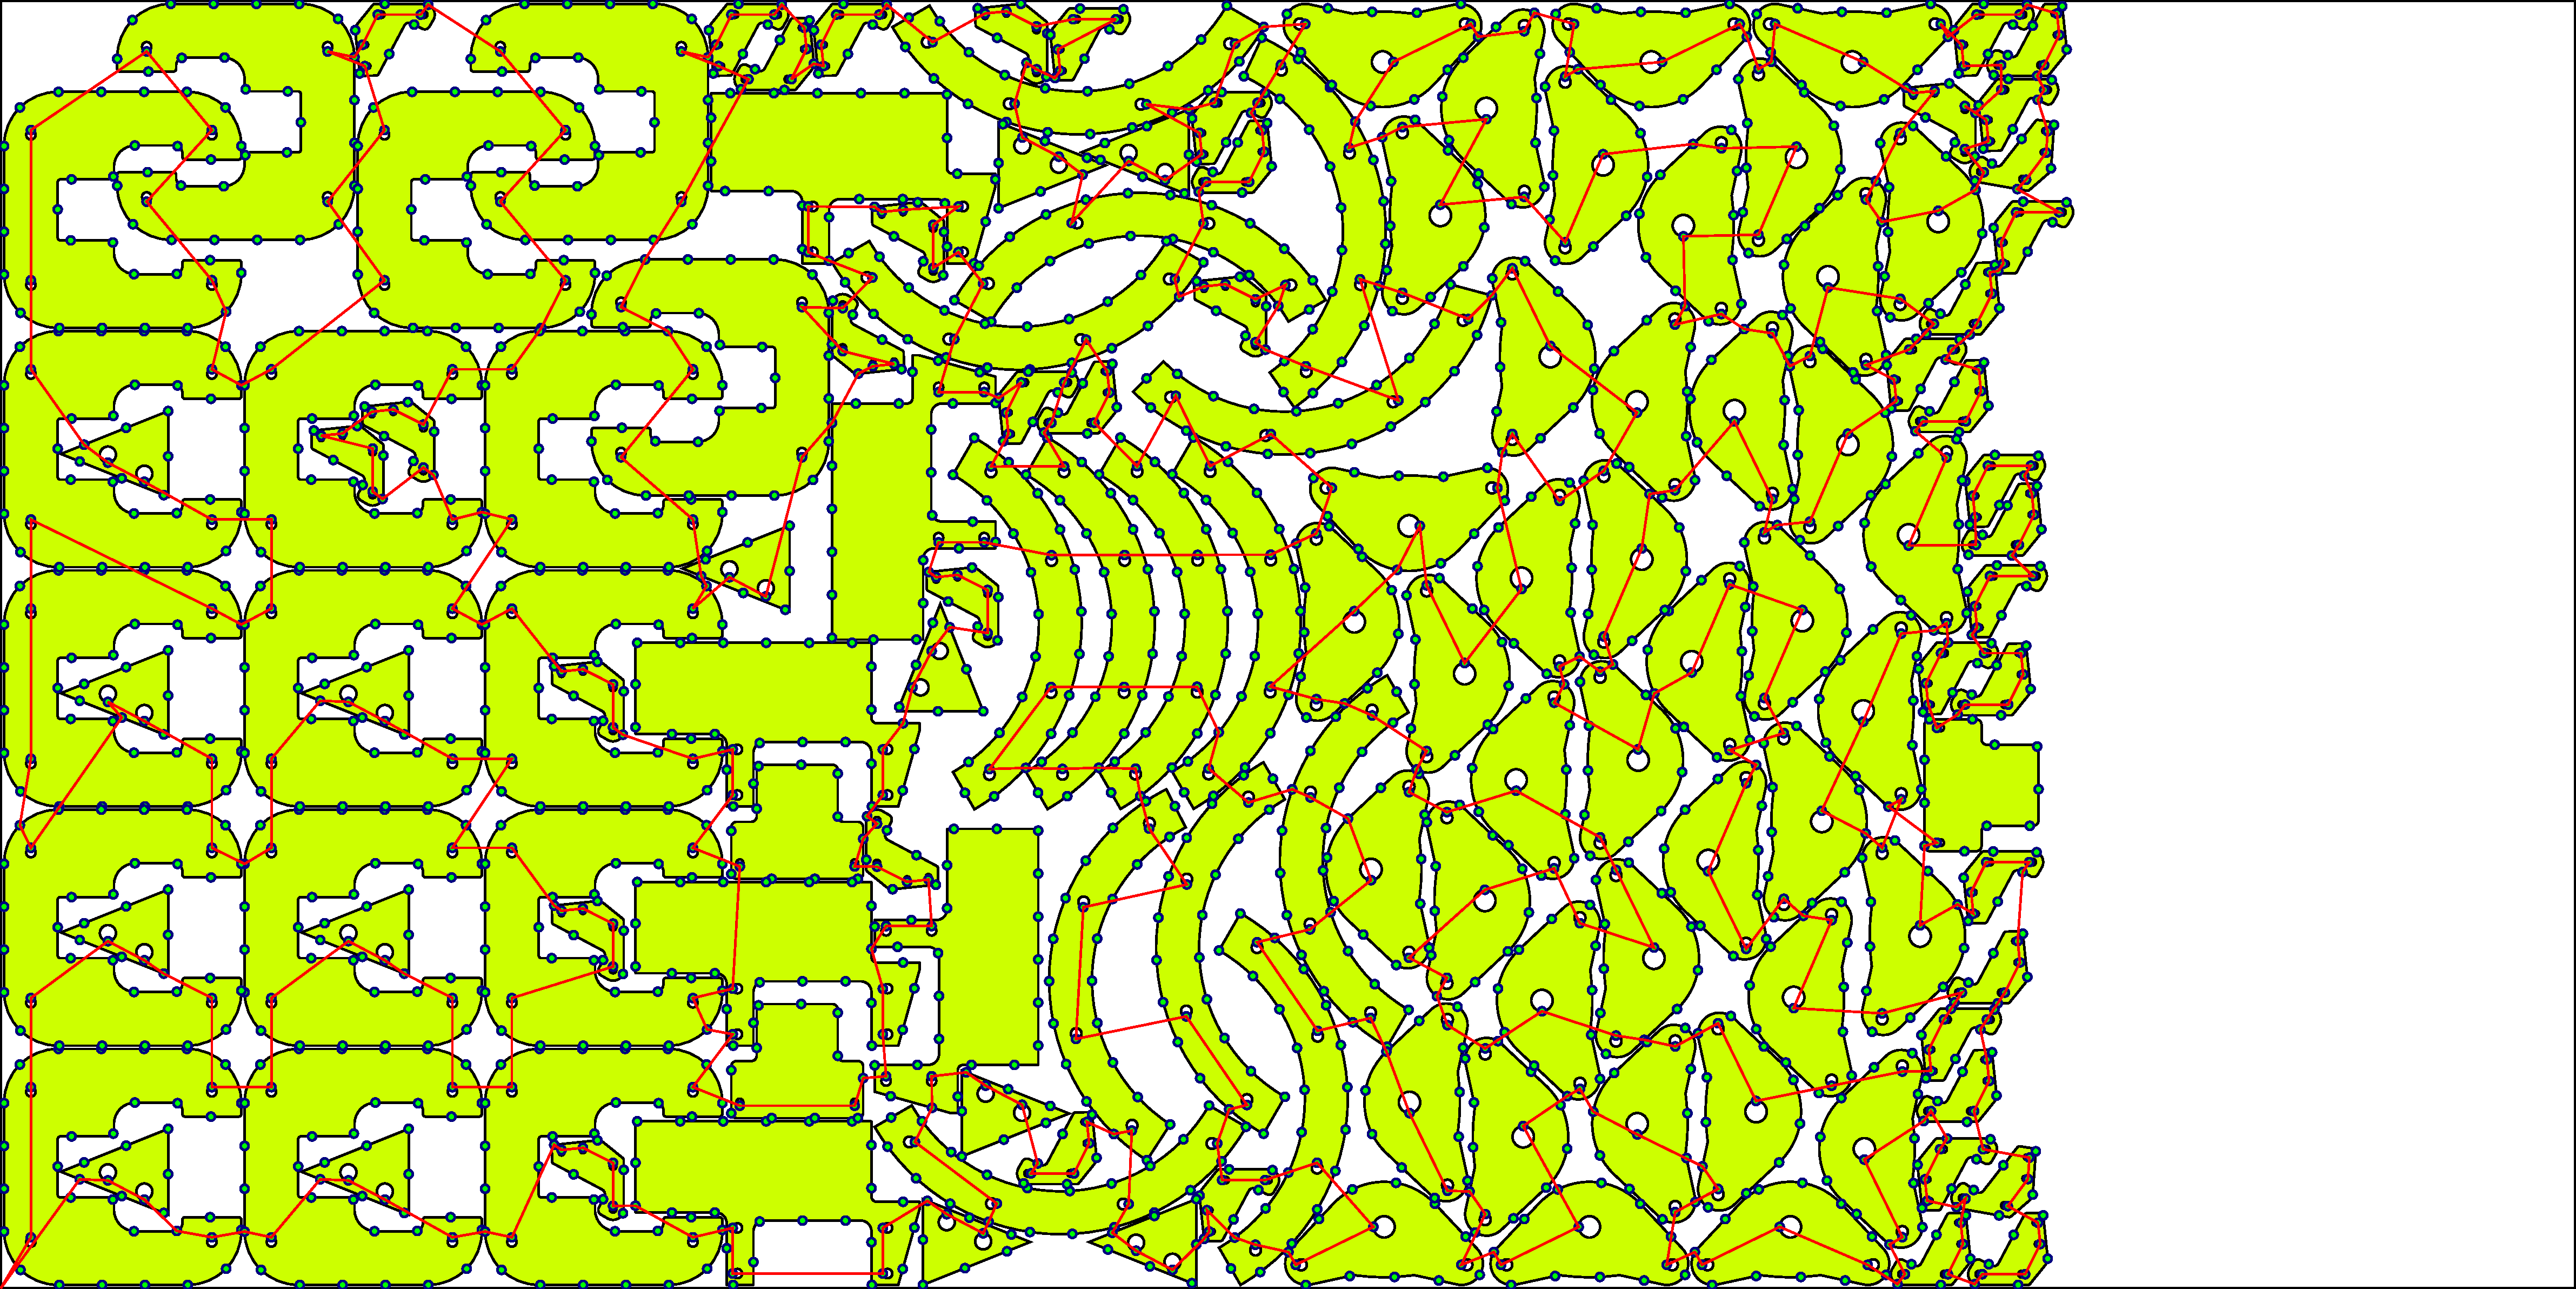
\includegraphics[width=0.95\textwidth]{ufa/b.pcglns.pdf}
  }
  \caption{Решения задач PCGTSP большой размерности}
  \label{fig:pcgtsp.ufa}
\end{figure}

\begin{table}
  \centering
  \caption{Результаты решения задач PCGTSP большой размерности}
  \label{tab:pcgtsp.ufa}
  \begin{tabular}{*{5}{|r}|}
    \hline
    Узлов & Контуров & Время, c & $\mathcal L$, мм & Оценка \\
    \hline
    2062 & 424 & 1533 & 24496 & 40.29\% \\
    2253 & 621 & 3181 & 34705 & 25.41\% \\
    \hline
  \end{tabular}
\end{table}
